\documentclass[12pt]{article}
\usepackage[margin=1in]{geometry}
\usepackage{graphicx}
\usepackage{tabulary}
\usepackage{times}
\usepackage[T1]{fontenc}
\usepackage{textcomp}
\usepackage{titlesec}
\usepackage{hanging}
\usepackage{url}
\newcommand{\sectionbreak}{\clearpage}

\graphicspath{ {img/} }

\begin{document}

\begin{titlepage}
  \begin{center}
    \vspace*{1cm}
    \huge\textbf{{Integrating IPv6 into the CPE464 Lab Curriculum}}

    \vspace{1.5cm}

    \begin{figure}[ht!]
      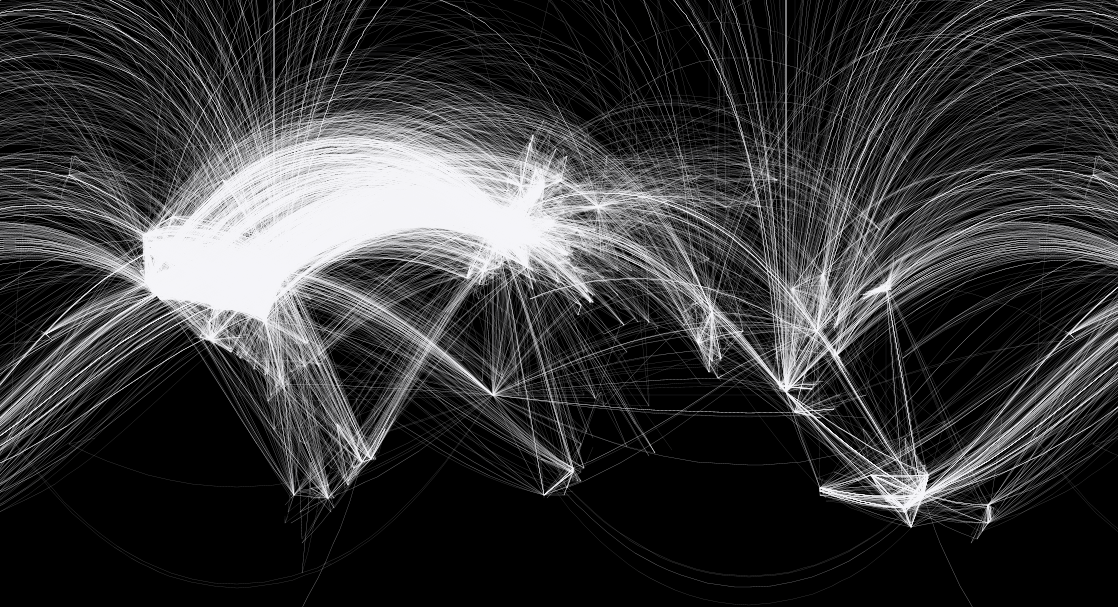
\includegraphics[width=1\textwidth]{internet_map.png}
      \label{fig:internet_map}
    \end{figure}

    \vfill
    \large{
      Jacob Hladky\\
      California Polytechnic State University\\
      San Luis Obispo, CA\\
      \texttt{jhladky@calpoly.edu}
    }

    \vspace{1cm}

    \today   
  \end{center}
\end{titlepage}

\pagenumbering{roman}

\tableofcontents

\listoffigures
\bigskip
\begin{hangparas}{1.35in}{1}
\hspace{0.25in}\textit{Title Image} \hspace{0.25in} A map of the IPv6 world. The image is a result of mapping the connections between the 100,000 most central IPv6 nodes on the Internet.
\end{hangparas}

\begingroup
\let\clearpage\relax
\listoftables
\endgroup
\clearpage

\pagenumbering{arabic}

\section{Introduction}
The Internet Protocol version 4 was standardized in 1981 by DARPA, a division of the Department of Defense focused on developing cutting-edge technologies (Information Sciences Inst.). The protocol --- designed to connect every computer on the globe --- could address roughly 4 billion hosts, a number which seemed unbelieveably immense compared to the 200 or so computers on the Internet at the time (Computer History Museum).\\\\
On the 4th of July of this year the American Registry for Internet Numbers, which assigns Internet addresses (``IP addresses'') is predicted to exhaust its remaining IP addresses (Huston). Registries in Asia and Europe have already run out of their share of the ``address space''.  A replacement protocol -- version 6 -- was approved in 1998, but laid dormant for most of the 2000s (Deering \& Hinden). Now, IPv4 exhaustion has spurred rapid adoption. Figure~\ref{fig:v6_adoption} shows the skyrocketing IPv6 adoption rates. IPv6 is rapidly becoming relevant in both the consumer and enterprise sectors.

\begin{figure}[ht!]
  \centering
  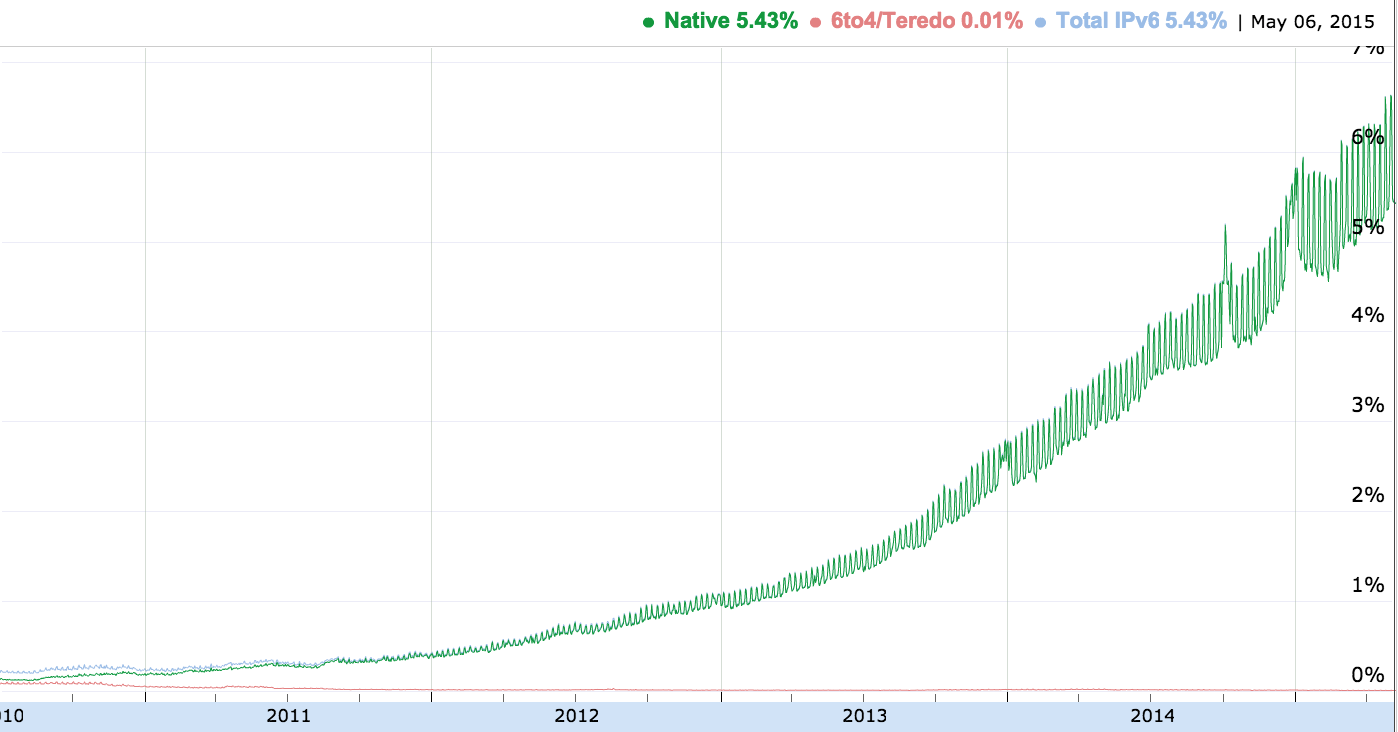
\includegraphics[width=0.65\textwidth]{v6_adoption.png}
  \caption{Percentage of users accessing \texttt{www.google.com} over IPv6}
  \label{fig:v6_adoption}
\end{figure}

\noindent Cal Poly students taking CPE464, Introduction to Computer Networks, will learn IPv4 in depth. In their accompanying lab section they will implement IPv4 on Cisco networking equipment. The CPE464 lecture will also cover IPv6, but the lab will not. This report will present research about the best way to integrate the teaching of IPv6 into the CPE464 lab curriculum.\\\\
This research can be broken into two parts. The first will address networking technologies that implement IPv6. The second will investigate various ways to integrate these technologies into the existing lab curriculum. This report will then select the optimal option from each and combine them to form a lesson plan, a recommendation on what technology to use and how to use it in the CPE464 lab.\\\\
The \textit{Methods} section of this report will summarize the areas of research that were looked into and what specific sources were researched in those areas. The \textit{Results} section will then present the research findings from each of the methods. The \textit{Conclusion} and \textit{Recommendations} sections will then detail an the best course of action derived from the research. Finally, a \textit{Glossary of Terms} will provide definitions for any unfamiliar terms used in this report.

\section{Methods}
In the course of researching this report I split the problem at hand, of how best to teach the concepts of IPv6 to CPE464 lab students, into two questions. The first: ``What technologies best show how IPv6 is different from IPv4?'' The second: ``What is the best way to integrate these technologies into the CPE464 lab curriculum?'' Correspondingly, I used two different methods of research, using the findings from each method to answer one of the two questions.\\\\
These two questions can be categorized respectively as a technical question and a pedagogical question. To answer the technical question I consulted internet research and to answer the pedagogical question I interviewed Dr. Hugh Smith. These two methods are further detailed in the two subsections below.

\subsection{Interview with Dr. Hugh Smith}
I interviewed Dr. Hugh Smith to find an answer to my second question. Dr. Smith is the professor currently teaching the CPE464 lecture and lab sections (he is also the main recipient of this report.) As one of the co-authors of the lab curriculum, Dr. Smith is uniquely qualified to assess which methods of presenting new lab material will be the most effective, and how they will meet each lab's unique constraints.\\\\
 My aim in talking to Dr. Smith was to determine exactly that: how the current CPE464 lab is structured, and how various IPv6 technologies might be integrated with the current labs. During the interview Dr. Smith suggested several different strategies to accomplish this, and detailed their pros and cons.

\subsection{Secondary Research}
I conducted secondary research online to answer my first question. I read several online manuals and briefs about various technologies that used IPv6 in a significant way. The technologies had to have two requirements to be researched:
\begin{itemize}
\item Significant presence in either the existing lab curriculum or in consumer networking
\item An existing and widely used IPv4 implementation
\end{itemize}
These requirements were to ensure that lab users would not be too unfamiliar with the new lab material, and so that old material could be used a template when writing new lab manuals and other documentation.

\subsubsection{Cisco: ``IPv6 Tunnel though a IPv4 Network''}
IPv6 and IPv4 networks are incompatible, and as a result it is necessary to pass IPv6 traffic through IPv4 networks so that they can communicate in the absence of a direct link (Cisco). This how-to guide details individual steps to accomplish this on Cisco iOS routers.

\subsubsection{Cisco: ``IPv6 Autoconfiguration''}
IPv6 addresses are very long and cumbersome to enter manually. Thus the protocol includes a feature where computers running IPv6 can pick their own address based on pre-determined factors inherent to the system (Donze). This white paper explains the process and lists several drawbacks.

\subsubsection{CircleID: ``DHCP for IPv4 vs. IPv6''}
This web article, intended for consumers, discusses how IPv6 addresses may be assigned through the Dynamic Host Configuration Protocol (DHCP). DHCP, optional in many IPv4 environments, is a crucial component of the new protocol (Donaldson).

\section{Results}
To evaluate the results of my interview with Dr. Smith I created a table summarizing the various methods of integrating new curriculum material mentioned in the interview. To evaluate the secondary results I used my own knowledge as a T.A. for the CPE464 lab section. I also created a decision matrix that assigns objective value to the different technologies. The secondary results will be described in a short summary, and then evaluated in the matrix based on the two criteria mentioned in the \textit{Methods} section.

\begin{figure}[ht!]
  \centering
  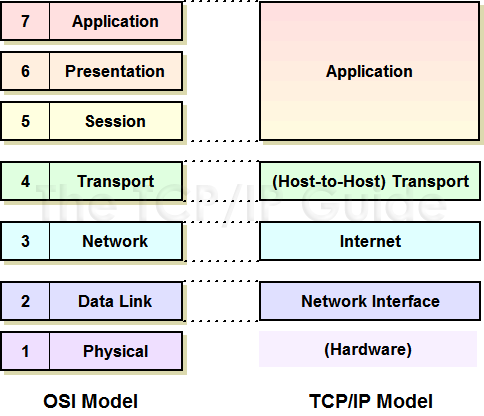
\includegraphics[width=0.4\textwidth]{the_stack.png}
  \caption{The Various Layers of the Network Stack}
  \label{fig:the_stack}
\end{figure}

\subsection{Interview with Dr. Hugh Smith}
Dr. Smith gave me a macro-level overview of the CPE464 curriculum. The lab curriculum is tightly coupled to the idea of the ``network stack'', shown in Figure~\ref{fig:the_stack}. Students start at the bottom of stack, and work their way gradually upward with each lab. There are 7 labs in total every quarter, and they are divided as follows:
\begin{itemize}
\item 2 labs on the link layer
\item 4 labs on the network layer
\item 1 lab on network security (session or presentation layer)
\end{itemize}

\noindent Dr. Smith suggested three different methods for integrating new material into the lab curriculum. The three methods are summarized in Table~\ref{table:method_summary} below.

\medskip
\begin{table}[h!]
  \centering
  \label{table:method_summary}
  \begin{tabulary}{\textwidth}{|L|L|R|R|}
    \hline
    \textbf{Method Name} & \textbf{Short Description} & \textbf{\# Labs Required} & \textbf{Mins. Required Per Lab} \\ \hline\hline
    Multiple & Whenever an IPv4 technology is used, also use the corresponding IPv6 variant & 6-7 & 30-40 \\ \hline
    Single & Add a new lab focusing entirely on IPv6. & 1 & All (180) \\ \hline
    Double & Split two labs between IPv4 and IPv6. & 2 & 90 \\ \hline
  \end{tabulary}
  \caption{Summary of methods for integrating new material into CPE464 lab}
\end{table}

\noindent The multiple method requires the most work. About 30 minutes of material would have to be removed from each lab to make room for the new IPv6 material. However, the new IPv6 material would already have been implemented using IPv4. Thus, labs constructed in this style have a high potential to become monotonous and repetitive for students. One significant advantage of this method is the wide range of exposure it would offer to IPv6 technologies.\\\\
The single method simply fills what was a week for students to do make-up lab work with a new lab. No re-factoring of existing curriculum is required, but students will not be exposed to IPv6 until late in the quarter, as the current labs are tightly integrated and must be completed in a certain order.\\\\
The double method is a compromise between the multiple and single methods. Only two labs are re-factored, but much more information is removed. This information could then either be removed completely from the curriculum or moved to a lab at the end. This method, like the multiple method, provides good exposure to IPv6, but possibly at the expense of other important network concepts.

\begin{figure}[ht!]
  \centering
  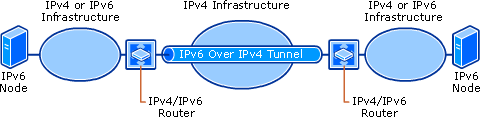
\includegraphics[width=0.7\textwidth]{v6_tunneling.png}
  \caption{Simplified diagram of how IPv6 tunneling works.}
  \label{fig:v6_tunneling}
\end{figure}

\subsection{Cisco: ``IPv6 Tunnel though a IPv4 Network''}
IP Tunneling is ubiquitous in networking, and IPv4-only tunneling is a crucial component of the Virtual Private Network (VPN), a widely used enterprise technology. Although it is not currently covered, students can be easily familiarized with IP Tunneling during lecture, as the core concept is easy to grasp. Figure~\ref{fig:v6_tunneling} shows how tunneling works on the network level.

\subsection{Cisco: ``IPv6 Autoconfiguration''}
IPv6 auto-configuration is a feature unique to the new protocol, and thus this technology suffers when compared IPv4, which has no comparable feature. Although some custom implementations exist which do the same thing, students are not likely to be familiar with them.

\subsection{CircleID: ``DHCP for IPv4 vs. IPv6''}
DHCP is used everyday by consumers, and is already covered in lecture, so it receives a very high familiarity score. However it suffers when used as a comparison protocol because its IPv6 implementation is \textit{too} similar to its v4 implementation. The commands and concepts used in both versions are nearly identical, and thus not useful for demonstrating IPv6.

\medskip
\begin{table}[h!]
  \centering
  \label{table:dec_matrix}
  \begin{tabulary}{\textwidth}{|L|C|C|C|}
    \hline
    Technology & Familiarity Score (0-9) & IPv4 Parallel Score (0-9) & Total Score (0-18) \\ \hline\hline
    Tunneling          & 7 & 7 & 14 \\ \hline
    Auto-configuration & 4 & 2 & 6 \\ \hline
    DHCP               & 9 & 4 & 13 \\ \hline
  \end{tabulary}
  \caption{Decision matrix for selecting the best IPv6 technology}
\end{table}

\section{Conclusions}
All three methods of presenting IPv6 have drawbacks, but while analyzing the results it became clear that one drawback was significantly more important than the others: the amount of work that would be required to re-tool the entire lab curriculum. Both the multiple and double options, while offering significant exposure to IPv6, require changing other labs, and could possibly result in a reshuffling of the lab curriculum. The interview with Dr. Smith also brought to light how tightly coupled the CPE464 individual labs are, and that reshuffling them could cause significant confusion in both students and the T.A.s who help them. Thus, the best option is a single, monolithic lab that will be added as the last lab students complete in the quarter.\\\\
For the faculty, this is the most ``efficient'' option, as it results in the most new material from the least effort spent on re-factoring. For the students, a single extra lab is a net increase in knowledge.\\\\
On a similar note, the IPv6 technology that stands out is Tunneling. Auto-configuration is too obscure, and would require a genuine intellectual leap for many students because of its newness as a protocol. DHCP is common, but too easy. IP tunneling, which scored highest on the decision matrix, finds a middle path between these two extremes.\\\\
These results provide answers to the two sub-questions presented in the \textit{Methods} section, and now a ``lesson-plan'' can be presented that combines both results. This report thus recommends the addition of a single new lab, in the place of the current lab make-up week, which teaches students how IPv6 works by means of having them implement an IPv6 tunnel, following the instructions in the Cisco guide.

\section{Recommendations}
A single new lab should be added to the lab curriculum, with no modification to the other labs. The lab should teach IPv6 by having students implement an IPv6 tunnel through an existing IPv4 network. The students should follow the instructions presented in the Cisco guide ``IPv6 tunnel through an IPv4 network.''

\section{Glossary of Terms}

\begin{itemize}
\item[] \textbf{Computer Network} --- A collection of computers that can all talk to each other
\item[] \textbf{DHCP} --- The Dynamic Host Configuration Protocol. A method for a computer to automatically get an IP address without knowing anything about the network it's on.
\item[] \textbf{Host} --- A computer on a network
\item[] \textbf{iOS} --- The operating system running on Cisco network devices. Cisco iOS predates Apple's iOS running on iPhones.
\item[] \textbf{IP Address} --- A number that uniquely identifies a computer on a network
\item[] \textbf{IP Tunneling} --- Running traffic from some network A  through another network B where B can't see A's traffic
\item[] \textbf{IPv4} --- The Internet Protocol, version 4. Dominant network protocol for the world for the past 30 years.
\item[] \textbf{IPv6} --- The Internet Protocol, version 6. Replacement protocol for IPv4
\item[] \textbf{IPv6 Autoconfiguration} --- A means for a computer to automatically get an IPv6 address without talking to a DHCP server or assigning one manually.
\item[] \textbf{Network Stack} --- A collection of modular, inter-operating protocols designed to move data from physical transmission, \textit{e.g.} cables and Wi-Fi Access Points, to the user and back.
\item[] \textbf{Network Traffic} --- Communication between hosts on a network
\item[] \textbf{VPN} --- Virtual Private Network. A technology often used by large corporations to enable employees to connect to the office network while at home.
\end{itemize}

\section{Works Cited}

\begin{hangparas}{0.25in}{1}
Cisco. ``IPv6 Tunnel through an IPv4 Network.'' Cisco, 10 Aug. 2006. Web. 06 May 2015. <\url{http://www.cisco.com/c/en/us/support/docs/ip/ip-version-6/25156_ipv6tunnel.html}>.\\

Computer History Museum. ``Computer History Museum.'' Computer History 1980s. Computer History Museum, 2004. Web. 06 May 2015. <\url{http://www.computerhistory.org/internet_history/internet_history_80s.html}>.\\

Deering, S., and R. Hinden. Internet Protocol, Version 6 (IPv6) Specification. RFC 2460. N.p.: Internet Society, 1998. Print\\

Donaldson, Richard. ``DHCP for IPv4 vs. IPv6 - What You Need to Know.'' CircleID. N.p., 02 June 2011. Web. 06 May 2015. <\url{http://www.circleid.com/posts/dhcp_for_ipv4_vs_ipv6_what_you_need_to_know/}>.\\

Donze, Francois. ``IPv6 Autoconfiguration.'' The Internet Protocol Journal 7.2 (2004): n. pag. Web. 6 May 2015. <\url{http://www.cisco.com/web/about/ac123/ac147/archived_issues/ipj_7-2/ipv6_autoconfig.html}>.\\

Huston, Geoff. ``IPv4 Address Report.'' IPv4 Address Report. N.p., 06 May 2015. Web. 06 May 2015. <\url{http://www.potaroo.net/tools/ipv4/}>.\\

Information Sciences Institute. INTERNET PROTOCOL DARPA INTERNET PROGRAM PROTOCOL SPECIFICATION. RFC 791. Arlington: Defense Advanced Research Projects Agency, 1981. Print.
\end{hangparas}

\begingroup
\let\clearpage\relax

\bigskip
\section{Figures Cited}

\begin{hangparas}{0.25in}{1}
Title Picture. Visualization with 100k Connections. Digital image. VISUALIZING THE INTERNET. DTU 02817, n.d. Web. 6 May 2015. <\url{http://www.olivergroth.dk/site/images/map_100k.png}>.\\

Figure~\ref{fig:v6_adoption}. IPv6 Adoption. Digital image. IPv6 -- Google. Google Inc., 6 May 2015. Web. 6 May 2015. <\url{https://www.google.com/intl/en/ipv6/statistics.html}>.\\

Figure~\ref{fig:the_stack}. Kozierok, Charles MM. OSI Reference Model and TCP/IP Model Layers. Digital image. The TCP/IP Guide. N.p., 20 Sept. 2005. Web. 6 May 2015. <\url{http://www.tcpipguide.com/free/diagrams/tcpiplayers.png}>.\\

Figure~\ref{fig:v6_tunneling}. Router-to-Router Tunneling. Digital image. IPv6 Transition Technologies (TechRef). Microsoft Inc., 7 Jan. 2009. Web. 6 May 2015. <\url{https://i-technet.sec.s-msft.com/dynimg/IC197206.gif}>.
\end{hangparas}

\bigskip
\section{Tables Cited}

\begin{hangparas}{0.25in}{1}
Table~\ref{table:method_summary}. Hladky, Jacob D. ``Summary of Methods for Integrating New Material into CPE464 Lab.'' pdfTeX 3.14 (Tex Live 2013/Debian) \\

Table~\ref{table:dec_matrix}. Hladky, Jacob D. ``Decision Matrix for Selecting the Best IPv6 Technology.'' pdfTeX 3.14 (Tex Live 2013/Debian)
\end{hangparas}

\endgroup

\end{document}



